\begin{figure}[ht]
   \centering
   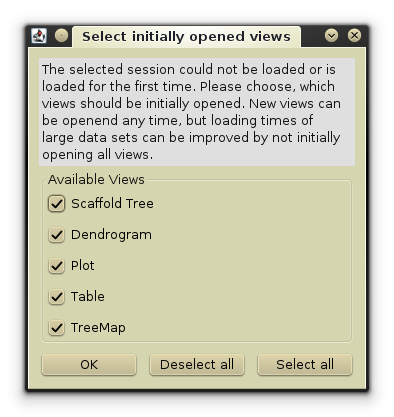
\includegraphics[width=.35\textwidth]{images/sh_initial_views.png}
   \caption{Selecting initially opened views}
   \label{fig:initial_views}
\end{figure}

When opening a session for the first time, the dialog shown in \figref{fig:initial_views} allows you to select the views that should be opened at start-up. Please note that new views can be created later at any time. However, for large datasets or in case of limited resources it is advisable to select only the required views and open additional views, e.g., for smaller subsets (see \secref{sec:scaffoldhunter:subsetmanagement}), on demand.
This reduces the loading times and memory requirements significantly.